\documentclass[10pt, a4paper,spanish]{article}
\usepackage[utf8]{inputenc}

\usepackage{hyperref}

\usepackage[T1]{fontenc}

\usepackage[hmarginratio=1:1,top=32mm,columnsep=20pt]{geometry}
\usepackage[hang, small,labelfont=bf,up,textfont=it,up]{caption}


\usepackage{graphicx}
\graphicspath{ {images/} }

\usepackage{abstract}
\renewcommand{\abstractnamefont}{\normalfont\bfseries}
\renewcommand{\abstracttextfont}{\normalfont\small\itshape}

\usepackage{titlesec}
\renewcommand\thesection{\Roman{section}}
\renewcommand\thesubsection{\Roman{subsection}}
\titleformat{\section}[block]{\large\scshape\centering}{\thesection.}{1em}{}
\titleformat{\subsection}[block]{\large}{\thesubsection.}{1em}{}


\usepackage{fancyhdr}
\pagestyle{fancy}
\fancyhead{}
\fancyfoot{}
\fancyhead[C]{ \today \ $\bullet$ Minería de Datos $\bullet$ Multicomparación de Clasificadores}
\fancyfoot[RO]{\thepage}

%-------------------------------------------------------------------------------
%	TITLE SECTION
%-------------------------------------------------------------------------------

\title{\vspace{-15mm}\fontsize{24pt}{10pt}\selectfont\textbf{Multicomparación de \\ Clasificadores}} % Article title

\author{Sergio García Prado}
\date{\today}

%-------------------------------------------------------------------------------

\begin{document}

	\maketitle % Insert title

	\thispagestyle{fancy} % All pages have headers and footers

%-------------------------------------------------------------------------------
%	ABSTRACT
%-------------------------------------------------------------------------------

	\begin{abstract}
		\noindent
	\end{abstract}

%-------------------------------------------------------------------------------
%	TEXT
%-------------------------------------------------------------------------------

	\section{Introducción}

        \paragraph{}
		La comparación consistirá en dos partes principales: la primera de ellas se basa en un Test de Signos sobre 2 de los clasificadores, (SVM y J48) para todos los conjuntos de datos, mientras que la segunda parte se refiere a la realización de un Ranking en el cuál participarán todos los clasificadores.

		\paragraph{}
		Para la realización de estas pruebas se ha utilizado Weka, una plataforma de software para el aprendizaje automático y la minería de datos escrita en Java, desarrollada en la Universidad de Waikato y distribuida como Software Libre.

		\paragraph{}
		Por lo tanto, lo primero es describir tanto los clasificadores como los conjuntos de datos que se utilizarán en los tests de clasificación:

		\subsection{Clasificadores}

			\begin{itemize}
				\item \textbf{SVM con kernel lineal}: Las máquinas de vector soporte son una técnica aprendizaje supervisado. Este modelo representa los puntos de muestra en el espacio, separando las clases en  subespacios lo más amplios posibles mediante un hiperplano de separación definido como el vector entre los puntos de las clases, mas cercanos al que se llama vector soporte. En este caso se ha utilizado un kernel lineal.

				\item \textbf{3-NN}: El método de los k vecinos más próximos es un método de clasificación supervisada no paramétrico. Estima el valor de la función de densidad de probabilidad o directamente la probabilidad a posteriori de las muestras para calcular los k puntos medios. En este caso se ha utilizado 3 puntos.

				\item \textbf{Naive Bayes}: es un algoritmo de clasificación probabilístico basado en el teorema de Bayes y algunas hipótesis adicionales que facilitan la simplificación del problema. Estas hipótesis presuponen la independencia entre variables, de ahí es de donde proviene el apelativo \emph{naive (ingenuo)} ya que esta presuposición no siempre es cierta. Es un clasificador que utiliza aprendizaje supervisado y utiliza el método de máxima verosimilitud.

				\item \textbf{J48}: es un algoritmo cuya función es generar un árbol de decisión. Su nombre original es \emph{C4.5} pero la implementación de Weka se denomina \emph{J48}. Para generar el árbol de decisión el árbol basa la selección de atributos en cada nodo según la entropía de los mismos con respecto a la clases en la que se desea clasificar las muestras. Es por tanto un algoritmo de aprendizaje supervisado.
			\end{itemize}

		\subsection{Conjuntos de Datos}

			\begin{enumerate}
				\item \textbf{Arrhythmia}: 452 muestras con 279 atributos y 16 clases.
				\item \textbf{Diabetes}: 768 muestras con 8 atributos y 2 clases.
				\item \textbf{Glass}: 214 muestras con 9 atributos y 7 clases.
				\item \textbf{Ionosphere}: 351 muestras con 34 atributos y 2 clases.
				\item \textbf{Iris}: 150 muestras con 4 atributos y 3 clases.
				\item \textbf{Labor}: 57 muestras con 16 atributos y 2 clases.
				\item \textbf{Seeds}: 210 muestras con 7 atributos y 3 clases.
				\item \textbf{Segment Test}: 210 muestras con 19 atributos y 7 clases.
				\item \textbf{Soybean}: 683 muestras con 35 atributos y 19 clases.
				\item \textbf{Vote}: 435 muestras con 16 atributos y 2 clases.
			\end{enumerate}


	\section{Test de Signos: SVM y J48}

        \paragraph{}
		El test de signos se ha realizado sobre los 10 conjuntos de datos aplicando validación cruzada de 10 particiones. Lo que se pretende con este test es contar el número de victorias de cada clasificador y otorgarle la victoria al que más número de veces haya sido seleccionado ganador. Los resultados obtenidos han sido los siguientes (siendo el conjunto de datos $i$ el que se encuentra en dicha posición en el apartado anterior.):

		\hfill
		\begin{center}
			\begin{tabular}{ | c || c | c | c | c | c | c | c | c | c | c | }
				\hline
				Datos		& 1 	& 2		& 3 	& 4 	& 5 	& 6		& 7 	& 8 	& 9 	& 10 \\ \hline \hline
				Ganador		& SVM 	& SVM 	& J48 	& J48 	& SVM 	& SVM 	& SVM 	& J48 	& SVM 	& J48 \\
				\hline
			\end{tabular}
		\end{center}

		\paragraph{}
		Por lo tanto, los resultados de aplicar el test de signos son los siguientes:
		\[Victorias(J48) = 4\]
		\[Victorias(SVM) = 6\]
		Entonces podemos concluir que para los conjuntos de datos utilizados, obtiene más victorias, por lo tanto en promedio genera mejores resultados, el clasificador \textbf{SVM}.

	\section{Ranking}

		\begin{center}
			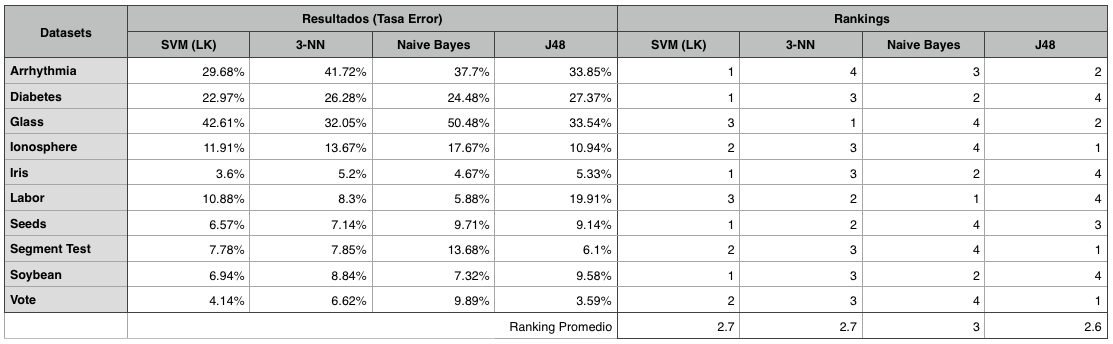
\includegraphics[width=\textwidth]{ranking-table}
		\end{center}

		\paragraph{}
		Realizaremos el test Friedman y el de Iman y Davenport:

		\paragraph{}
		Los valores que se utilizarán son los siguientes:

		$k = 4$, $N =10$,
		$\alpha = 0.05$,
		$\chi_{0.05,(2)}^2= 5.991$,
		$F_{0.05, (3,27)} =  2.960$

		\paragraph{}
		Tenemos que calcular además el estadístico de Friedman:

		\[
		\chi_{F}^2 = \frac{12N}{k(k+1)}\Big[\displaystyle\sum_{j}R_{j}^2 - \frac{k(k+1)^2}{4}\Big] = \frac{120}{20}\Big[(1.7^2+ 2.7^2+3^2+2.6^2) - \frac{100}{4}\Big] = 6 * 0.94 = 5.64\]

		\paragraph{}
		El test de Friedman nos dice que no se rechaza la hipótesis nula por lo que no son significativamente diferentes. A pesar de ello, no es rechazada por muy poco, pero debido a la exigencia que pide este test ya sabemos que en el caso de Iman y Davenport tampoco será rechazada. A pesar de ello, realizaremos los cálculos:

		\paragraph{}
		Con este valor calculamos el estadístico necesario para el test de Iman y Davenport:

		\[F_{F}= \frac{(N-1)\chi_{F}^2}{N(k-1)-\chi_{F}^2} = \frac{9 * 5.64}{30-5.64} = 2.0837 \]

		\paragraph{}
		Puesto que el valor de $F_{F}$ no es mayor que el valor crítico de $F_{0.05, (3,27)}$ entonces no podemos rechazar la hipótesis nula, que consiste en asumir que los clasificadores son equivalentes.

		\paragraph{}
		Debido a que no son significativamente diferentes tanto con el test de Friedman (muy exigente) como con el de Iman y Davenport (menos exigente), no tiene sentido realizar el test post-hoc para conocer cuáles lo son ya que este test ya nos ha dicho que no lo es ninguno.


\end{document}
